\chapter{Phasen}
\section{Entwurf und Anforderungen}
\subsection{Funktionale Anforderungen}
\begin{itemize}
	\item Das System muss fähig sein zufällig eine Spielwelt mit Hindernissen zu generieren welche jedoch so platziert werden müssen dass sie immer überwindbar sind.
	\item Das System muss fähig sein das generierte Spielfeld durch das Bild nach links zu verschieben.
	\item Bei drücken der Leertaste muss das System die Spielfigur hüpfen lassen.
	\item Das System muss fähig sein einen Highscore in Abhängigkeit zur Spieldauer zu generieren. Der Highscore soll proportional zum Levelfortschritt berechnet werden und dauerhaft angezeigt werden. Hierbei soll der aktuelle Score und der Highscore der Spielesession getrennt angezeigt werden. Dieser wird nur solange gespeichert, bis das Spiel beendet wird.
	\item Das System muss fähig sein während des Spielens eine Hintergrundmusik abzuspielen, welche sich ständig wiederholt.
	\item Das System muss fähig sein beim Springen der Spielfigur, beim Aufkommen der Spielfigur und beim kollidieren der Spielfigur Effektsounds   wiederzugeben.
	\item Das System muss die Möglichkeit bieten bei Tastendruck das Spiel zu pausieren und wieder zu starten.
	\item Das System muss fähig sein eine Kollision der Spielfigur mit einem Hindernis zu erkennen, nach erkennen soll ein „Crash“ Sound abgespielt werden und sich die Spielfigur verändern.
	\item Das System muss fähig sein kontinuierlich die Schwierigkeit zu erhöhen. Die Schwierigkeit soll dadurch erhöht werden, dass das Spielfeld anfangs langsam nach links wandert und dies kontinuierlich immer schneller wird.
	\item Bei Beendigung des Spiels muss das System fähig sein das Spiel neu zu starten. 
	\item Das System muss auf einem Gerät mit Tastatur im Browser Chrome ablaufen.
\end{itemize}
\subsection{Nicht funktionale Anforderungen}
\begin{itemize}
	\item Das Spiel sollte intuitiv Bedienbar sein.
	\item Die Perfomarnce des Spiels sollte so gut sein, dass keine Frame Einbrüche vorkommen.
	\item Auch auf den weiterverbreiteten Browsern sollte das Spiel spielbar sein.
\end{itemize}
\subsection{Projektplan}
\begin{table}[h]
	\begin{tabular}{l|l}
		\toprule
		\textbf{Datum}& \textbf{Aufgabe}\\
		\midrule
		19.10.2016 & Einführung in jeweilige Projekte der Gruppen 	\\ 
		21.10.2016 & Einführung in jeweilige Projekte der Gruppen	\\
		26.10.2016 & Anforderungen	\\ 
		02.11.2016 & Fertigstellung Präsentation, Ergebnispräsentation der Anforderungen \\
		04.11.2016 & Abgabe der Anforderungsspezifikation via Felix \\
		\bottomrule
	\end{tabular}
	\caption{Phase 1: Entwurf und Anforderungen}
\end{table}
\begin{table}[h]
	\begin{tabular}{l|l}
		\toprule
		\textbf{Datum}& \textbf{Aufgabe}\\
		\midrule
		09.11.2016 & Basis Implementierung 	\\ 
		16.11.2016 & Basis Implementierung + Level Design	\\
		23.11.2016 & Zwischenpräsentation der Implementierung	\\ 
		25.11.2016 & Abgabe: Zwischenstand der Implementation via Felix\\
		30.11.2016 & Level Design Verbesserungen \\
		07.12.2016 & Stabilität \& Bug fixing \\
		14.12.2016 & Ergebnispräsentation der Implementierung \\
		16.12.2016 & Abgabe Implementierungsergebnisses via Felix (Code Freeze) \\
		\bottomrule
	\end{tabular}
	\caption{Phase 2: Implementierung}
\end{table}
\begin{table}[h]
	\begin{tabular}{l|l}
		\toprule
		\textbf{Datum}& \textbf{Aufgabe}\\
		\midrule
		21.12.2016 & Test und Resultate Dokumentieren 	\\ 
		11.01.2017 & Ergebnispräsentation	\\
		13.01.2017 & Abgabe der Ergebnisse der Testphase	\\ 
		\bottomrule
	\end{tabular}
	\caption{Phase 3: Test}
\end{table}
\begin{table}[h]
	\begin{tabular}{l|l}
		\toprule
		\textbf{Datum}& \textbf{Aufgabe}\\
		\midrule
		18.01.2017 & Dokumentation 	\\ 
		25.01.2017 & Ergebnispräsentation Dokumentation	\\
		27.01.2017 & Projektvorstellung auf der Projektmesse	\\ 
		\bottomrule
	\end{tabular}
	\caption{Phase 4: Dokumentation und Präsentation}
\end{table}
\newpage
\subsection{Releaseplan}
\begin{longtable}{l|l|p{10cm}}
	\toprule
	\textbf{Version} & \textbf{Datum} & \textbf{Inhalt}\\
	\midrule
	1.0.0 & 09.11.16 & Spiel ist startfähig mit passendem Hintergrund und Spielfigur\\ 
	1.1.0 & 16.11.16 & Automatischer Bildlauf und springen ist möglich\\
	1.2.0 & 30.11.16 & Beinhaltet: Zufallsgenerierte Objekte(Hindernisse) mit unendlichem Level\\ 
	1.3.0 & 07.12.16 & Highscore, Hintergrundlied, Sound beim Springen\\
	1.4.0 & 14.12.16 & Zeitbasierte Geschwindigkeit (Bildlauf)\\
	1.5.0 & 21.12.16 & Erfolgreicher Test mit behobenen Fehlern\\
	\bottomrule
 	\caption{Releaseplan}
\end{longtable}
Beim Releaseplan haben wir uns auf eine Versionierung des Programms mit aufsteigenden Nummern geeinigt. Die Erste Nummer steht hierbei für die Grundlegende Programmversion. Die Zweite für wichtige Updates und die Dritte für Bugfixes zwischendurch. Zu jeweiligen Version haben wir ein Fertigstellungsdatum festgelegt und den dann erforderlichen Inhalt festgelegt.
\newpage
\section{Implementation}
\subsection{Erfüllte Anforderungen}
\begin{itemize}
	\item Das System muss fähig sein zufällig eine Spielwelt mit Hindernissen zu generieren welche jedoch so platziert werden müssen dass sie immer überwindbar sind.
	\item Das System muss fähig sein das generierte Spielfeld durch das Bild nach links zu verschieben.
	\item Bei drücken der Leertaste muss das System die Spielfigur hüpfen lassen.
	\item Das System muss die Möglichkeit bieten bei Tastendruck das Spiel zu pausieren und wieder zu starten.
	\item Das System muss fähig sein kontinuierlich die Schwierigkeit zu erhöhen. Die Schwierigkeit soll dadurch erhöht werden, dass das Spielfeld anfangs langsam nach links wandert und dies kontinuierlich immer schneller wird.
	\item Bei Beendigung des Spiels muss das System fähig sein das Spiel neu zu starten. 
	\item Das System muss auf einem Gerät mit Tastatur im Browser Chrome ablaufen.
\end{itemize}

\subsection{Nicht erfüllte Anforderungen}
\begin{itemize}
	\item Das System muss fähig sein eine Kollision der Spielfigur mit einem Hindernis zu erkennen, nach erkennen soll ein „Crash“ Sound abgespielt werden und sich die Spielfigur verändern.
	\item Das System muss fähig sein einen Highscore in Abhängigkeit zur Spieldauer zu generieren. Der Highscore soll proportional zum Levelfortschritt berechnet werden und dauerhaft angezeigt werden. Hierbei soll der aktuelle Score und der Highscore der Spielesession getrennt angezeigt werden. Dieser wird nur solange gespeichert, bis das Spiel beendet wird.
	\item Das System muss fähig sein während des Spielens eine Hintergrundmusik abzuspielen, welche sich ständig wiederholt.
	\item Das System muss fähig sein beim Springen der Spielfigur, beim Aufkommen der Spielfigur und beim kollidieren der Spielfigur Effektsounds   wiederzugeben.
\end{itemize}
\newpage
\subsection{Das Spiel}
Hier werden zwei Screenshots des derzeitigen Spiels dargestellt. In der Abbildung \ref{pic:start} zu sehen ist der Start Bildschirm des Spiels. Hier gibt es verschiedene Auswahl Möglichkeiten. In der Abbildung \ref{pic:spiel} zu sehen ist der derzeitige Stand des Spiels.
\begin{figure}[htb]
	\centering
	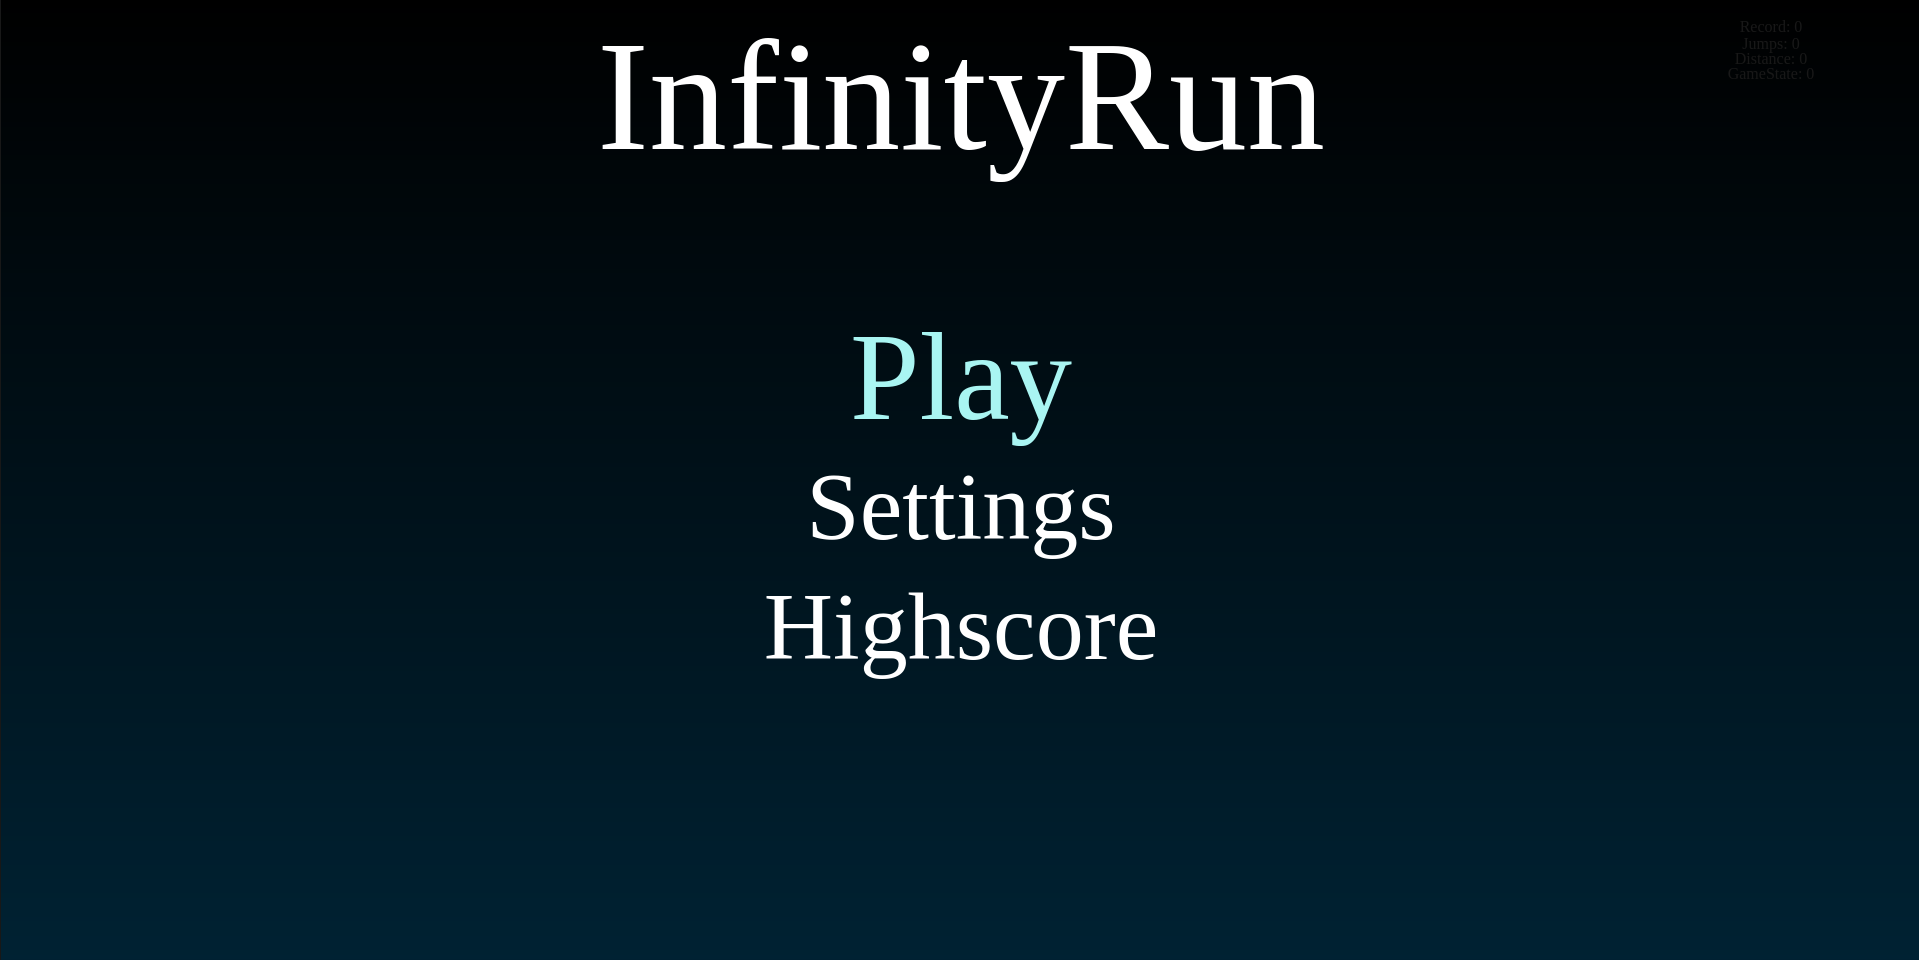
\includegraphics[scale=0.22]{content/pictures/start.png}
	\caption{Start Bildschirm}
	\label{pic:start}
\end{figure}
\begin{figure}[htb]
	\centering
	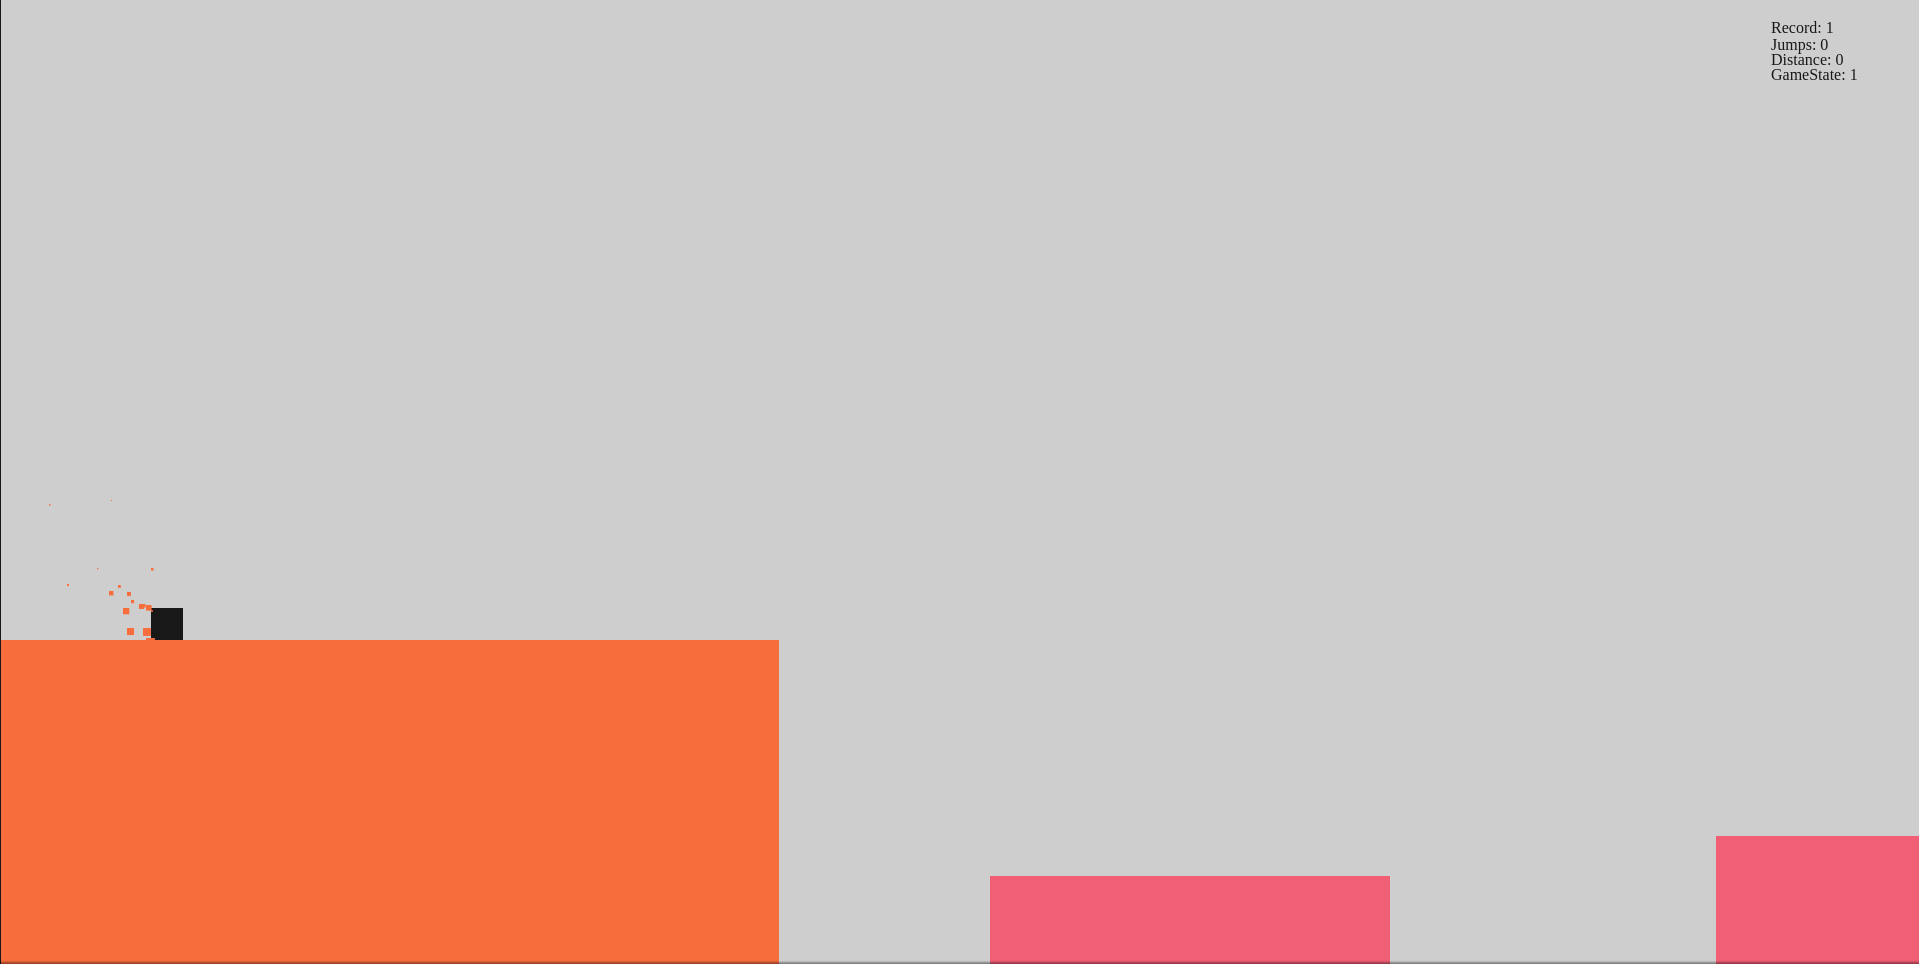
\includegraphics[scale=0.22]{content/pictures/spiel.png}
	\caption{Das Spiel}
	\label{pic:spiel}
\end{figure}
\newpage
\subsection{Bibliothek}
Bei der Erstellung des Spiels greifen wir auf eine JavaScript Bibliothek Namens ``Sketch.js'' zurück.
Das Sketch.js Framework ermöglicht es uns den Code vereinfacht und lesbarer zu schreiben. 
Beispiel wie Sketch.js funktioniert:

\lstset{language=java}
\begin{lstlisting}[frame=single]
function start() 
{
	context.now = +new Date();
    context.running = true;
}
        
function stop() 
{
	context.running = false;
}
        
function toggle() 
{       
	( context.running ? stop : start )();
}
        
function clear() 
{        
	if ( is2D )
        context.clearRect( 0, 0, context.width, context.height );
}
\end{lstlisting}
Quelle: \cite{sketch}
\subsection{Code}
\subsubsection{Framework initialisieren}
\lstset{language=java}
\begin{lstlisting}[frame=single]
var InfinityRun = Sketch.create({
fullscreen: true,
width: 640,
height: 360,
container: document.getElementById('container')
});
\end{lstlisting}
\subsubsection{Spieler initialisieren}
\lstset{language=java}
\begin{lstlisting}[frame=single]
Player.prototype.update = function() {
// Gravity 
this.velocityY += 1;
this.setPosition(this.x + this.velocityX, this.y + this.velocityY);

if (this.y > InfinityRun.height || this.x + this.width < 0) 
{
	this.x = 150;
	this.y = 50;
	this.velocityX = 0;
	this.velocityY = 0;
	InfinityRun.jumpCount = 0;
	InfinityRun.acceleration = 0;
	InfinityRun.accelerationTweening = 0;
	InfinityRun.scoreColor = '#181818';
	InfinityRun.platformManager.maxDistanceBetween = 350;
	InfinityRun.platformManager.updateWhenLose();
}

if ((InfinityRun.keys.UP || InfinityRun.keys.SPACE || InfinityRun.keys.W || InfinityRun.dragging) && this.velocityY < -8) 
{
	this.velocityY += -0.75;
}
};
\end{lstlisting}
\subsubsection{Erstellen der Spielebene}
\lstset{language=java}
\begin{lstlisting}[frame=single]
Player.prototype.update = function() {
function PlatformManager() 
{

	this.maxDistanceBetween = 300;

	this.colors = ['#2ca8c2', '#98cb4a', '#f76d3c', '#f15f74', '#5481e6'];

//first 3 Platforms execept the Starter Platform
	this.first = new Platform({
	x: 300,
	y: InfinityRun.width / 2,
	width: 400,
	height: 70
})

this.second = new Platform
({
	x: (this.first.x + this.first.width) + random(this.maxDistanceBetween - 150, this.maxDistanceBetween),
	y: random(this.first.y - 128, InfinityRun.height - 80),
	width: 400,
	height: 70
})

this.third = new Platform
({
	x: (this.second.x + this.second.width) + random(this.maxDistanceBetween - 150, this.maxDistanceBetween),
	y: random(this.second.y - 128, InfinityRun.height - 80),
	width: 400,
	height: 70
})
	this.first.height = this.first.y + InfinityRun.height;
	this.second.height = this.second.y + InfinityRun.height;
	this.third.height = this.third.y + InfinityRun.height;
	this.first.color = randomChoice(this.colors);
	this.second.color = randomChoice(this.colors);
	this.third.color = randomChoice(this.colors);
	this.colliding = false;
	this.platforms = [this.first, this.second, this.third];
}
\end{lstlisting}
\subsubsection{Update der Plattformen}
\lstset{language=java}
\begin{lstlisting}[frame=single]
PlatformManager.prototype.update = function() 
{
	this.first.x -= 3 + InfinityRun.acceleration;
	if (this.first.x + this.first.width < 0) 
	{
		this.first.width = random(450, InfinityRun.width + 200);
		this.first.x = (this.third.x + this.third.width) + random(this.maxDistanceBetween - 150, this.maxDistanceBetween);
		this.first.y = random(this.third.y - 32, InfinityRun.height - 80);
		this.first.height = this.first.y + InfinityRun.height + 10;
		this.first.color = randomChoice(this.colors);
	}

	this.second.x -= 3 + InfinityRun.acceleration;
	if (this.second.x + this.second.width < 0) 
	{
		this.second.width = random(450, InfinityRun.width + 200);
		this.second.x = (this.first.x + this.first.width) + random(this.maxDistanceBetween - 150, this.maxDistanceBetween);
		this.second.y = random(this.first.y - 32, InfinityRun.height - 80);
		this.second.height = this.second.y + InfinityRun.height + 10;
		this.second.color = randomChoice(this.colors);
	}

	this.third.x -= 3 + InfinityRun.acceleration;
	if (this.third.x + this.third.width < 0) 
	{
		this.third.width = random(450, InfinityRun.width + 200);
		this.third.x = (this.second.x + this.second.width) + random(this.maxDistanceBetween - 150, this.maxDistanceBetween);
		this.third.y = random(this.second.y - 32, InfinityRun.height - 80);
		this.third.height = this.third.y + InfinityRun.height + 10;
		this.third.color = randomChoice(this.colors);
	}
};
\end{lstlisting}
\subsubsection{Update der Plattformen}
\lstset{language=java}
\begin{lstlisting}[frame=single]
    for (i = 0; i < this.platformManager.platforms.length; i++) 
    {
		if (this.player.intersects(this.platformManager.platforms[i])) 
		{
			this.collidedPlatform = this.platformManager.platforms[i];
			if (this.player.y < this.platformManager.platforms[i].y) 
			{
				this.player.y = this.platformManager.platforms[i].y;
				// Gravity after Collision with Platform
				this.player.velocityY = 0;
			}

			this.player.x = this.player.previousX;
			this.player.y = this.player.previousY;
			
			this.particles[(this.particlesIndex++) % this.particlesMax] = new Particle({
			x: this.player.x,
			y: this.player.y + this.player.height,
			color: this.collidedPlatform.color
});
\end{lstlisting}
\section{Test}
\section{Dokumentation \& Pr\"asentation}

